\scanpage{17}
\uline{Cas particuliers}

Supposons que $\forall i\in I$, \deleted{$\unsure{E_i|\Sigma_i}$ \unsure{est|soit} \unsure{rare|dense} dans $X$.} \inserted{on ait} (si $\Sigma_i^+\ \Sigma_i^-$ sont les deux comp. conn. de $X\setminus\Sigma_i$)

\deleted{Alors on \unsure{trouve} que}
\[
\begin{aligned}
\overline{\Sigma_i^+} &= \Sigma_i^+\cup E_i\\
\overline{\Sigma_i^-} &= \Sigma_i^-\cup E_i .
\end{aligned}
\]

Alors je dis qu'on a
\[
\overline{\Sigma_{12}}=\Sigma_{12}
% G01: two curved passes of the first cup; full-scan origin (946,783).
\mathbin{\vcenter{\hbox{
\begin{tikzpicture}[x=0.014cm,y=-0.014cm]
\useasboundingbox (0,0) rectangle (36,32);
\begin{scope}[shift={(-946,-783)}]
\draw[line width=0.65pt] (950,787) .. controls (949,803) and (953,810) .. (960,810) .. controls (976,812) and (979,800) .. (974,789);
\draw[line width=0.50pt] (950,788) .. controls (950,802) and (951,807) .. (959,808) .. controls (971,807) and (971,798) .. (968,790);
\end{scope}
\end{tikzpicture}}}} E_1\cup E_2
\]

% G02: shallow separator and downturned right endpoint; full-scan origin (300,888).
\figure{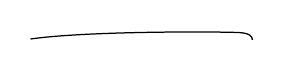
\begin{tikzpicture}[x=0.012cm,y=-0.012cm]
\useasboundingbox (0,0) rectangle (242,25);
\begin{scope}[shift={(-300,-888)}]
\draw[line width=0.45pt] (303,900) .. controls (359,892) and (483,892) .. (519,893) .. controls (535,893) and (538,897) .. (538,901);
\end{scope}
\end{tikzpicture}}

% slanted
\reversemarginpar
\margin{introduire la partition $\Pi_j=\{\deleted{\unsure{\Sigma}}E_j,\Sigma_j^+,\Sigma_j^-\}$
% G03: short dark wedge to the right of the closing brace in crop05.
% Its character, role, hand, and possible attachment to neighbouring text remain open.
\unsure{\begin{tikzpicture}[x=0.25mm,y=0.25mm,baseline=0pt]
\useasboundingbox (0,0) rectangle (3,4);
\fill (0,0) -- (0.4,3) -- (2.2,2) -- cycle;
\end{tikzpicture}}}
\normalmarginpar
\deleted{Supposons}

Soit $J\subset I$ tel que $I=J\amalg\{i\}$.

Consid\unsure{e|é}rons la partition
% G04: first Pi_J insertion and its curved guide. Fixed source origin (1218,1105).
\begin{tikzpicture}[x=0.010cm,y=-0.010cm,baseline=(live.base)]
\useasboundingbox (0,0) rectangle (180,130);
\node[anchor=base west,inner sep=0pt,outer sep=0pt] (added) at (0,58) {\inserted{$\Pi_J$}};
\node[anchor=base west,inner sep=0pt,outer sep=0pt] (live) at (70,115) {de};
\begin{scope}[shift={(-1218,-1105)}]
\draw[line width=0.40pt] (1282,1226) .. controls (1284,1204) and (1306,1196) .. (1338,1192) .. controls (1354,1189) and (1367,1188) .. (1370,1183);
\end{scope}
\end{tikzpicture}
$X$ \deleted{definie} definie par les $\deleted{\Sigma}E_j$ $(j\in J)$, \deleted{\unsure{et}} intersection des partitions
% G05: ternaires Pi_j and the long V-shaped guide; source origin (947,1345).
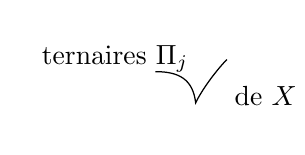
\begin{tikzpicture}[x=0.009cm,y=-0.009cm,baseline=(live.base)]
\useasboundingbox (0,0) rectangle (352,140);
\node[anchor=base west,inner sep=0pt,outer sep=0pt] (added) at (20,52) {\inserted{ternaires $\Pi_j$}};
\node[anchor=base west,inner sep=0pt,outer sep=0pt] (live) at (292,110) {de $X$};
\begin{scope}[shift={(-947,-1345)}]
\draw[line width=0.45pt] (1127,1407) .. controls (1161,1407) and (1180,1418) .. (1184,1451) .. controls (1193,1432) and (1214,1404) .. (1228,1390);
\end{scope}
\end{tikzpicture}
$(j\in J)$ definies par les $E_j$ $\unsure{\deleted{\in}|\deleted{E}|\notin}$ $(j\in J)$
\[
X=E_j\amalg\coprod_{\alpha\in\pi_0(X\setminus E_j)}\Sigma_j^\alpha
\]

-- c'est aussi la partition definie par celle de
% G06: detached baseline point before the first union, role and hand unresolved.
$\displaystyle \unsure{\mathord{
\begin{tikzpicture}[x=0.025cm,y=-0.025cm,baseline=0pt]
\useasboundingbox (0,0) rectangle (9,7);
\begin{scope}[shift={(-734,-1902)}]
\fill (735,1903) -- (741,1902) -- (741,1907) -- (735,1907) -- cycle;
\end{scope}
\end{tikzpicture}}}\bigcup_{j\in J}E_j$ en les $E_j$, et la partition
% G07: raised Pi_J ring and bent guide; source origin (752,1973).
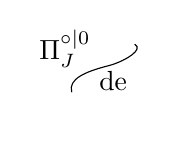
\begin{tikzpicture}[x=0.010cm,y=-0.010cm,baseline=(live.base)]
\useasboundingbox (0,0) rectangle (168,110);
\node[anchor=base west,inner sep=0pt,outer sep=0pt] (added) at (15,40) {\inserted{$\Pi_J^{\unsure{\circ|0}}$}};
\node[anchor=base west,inner sep=0pt,outer sep=0pt] (live) at (91,80) {de};
\begin{scope}[shift={(-752,-1973)}]
\draw[line width=0.40pt] (808,2055) .. controls (803,2038) and (826,2029) .. (852,2022) .. controls (870,2018) and (894,2005) .. (891,1997) -- (888,1994);
\end{scope}
\end{tikzpicture}
$\displaystyle X\setminus
% G08: literal cup and transverse upper stroke; source origin (1118,1976).
\mathop{\vcenter{\hbox{
\begin{tikzpicture}[x=0.009cm,y=-0.009cm]
\useasboundingbox (0,0) rectangle (69,70);
\begin{scope}[shift={(-1118,-1976)}]
\draw[line width=0.45pt] (1130,1980) .. controls (1125,1999) and (1126,2020) .. (1137,2034) .. controls (1152,2045) and (1170,2034) .. (1176,2014) .. controls (1180,2003) and (1177,1986) .. (1172,1980);
\draw[line width=0.40pt] (1123,1990) .. controls (1141,1990) and (1156,1988) .. (1168,1988);
\end{scope}
\end{tikzpicture}}}}\limits_{j\in J}E_j$ intersection des partitions binaires $\Pi_{J,j}^{\circ}$
% The upper ring's local circle/zero doubt is recorded also at this second occurrence.
% G09: inserted (j in J), live induites, and one continuous hooked guide.
% Fixed source origin (1234,2070); the guide supplies no extra prose parenthesis.
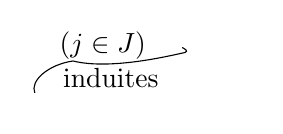
\begin{tikzpicture}[x=0.009cm,y=-0.009cm,baseline=(live.base)]
\useasboundingbox (0,0) rectangle (320,110);
\node[anchor=base west,inner sep=0pt,outer sep=0pt] (added) at (45,35) {\inserted{$(j\in J)$}};
\node[anchor=base west,inner sep=0pt,outer sep=0pt] (live) at (50,84) {induites};
\begin{scope}[shift={(-1234,-2070)}]
\draw[line width=0.40pt] (1244,2162) .. controls (1237,2145) and (1263,2122) .. (1298,2117) .. controls (1350,2130) and (1433,2110) .. (1456,2105) .. controls (1461,2103) and (1456,2100) .. (1452,2098);
\end{scope}
\end{tikzpicture}
% G10: U-subscript correction states and its long guide into the sur/X gap.
% Fixed source origin (311,2140); glyph/state alternatives carry no chronology.
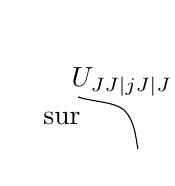
\begin{tikzpicture}[x=0.010cm,y=-0.010cm,baseline=(live.base)]
\useasboundingbox (0,0) rectangle (151,165);
\node[anchor=base west,inner sep=0pt,outer sep=0pt] (added) at (56,75) {\inserted{$U_{\unsure{\deleted{J}J|\deleted{j}J|J}}={}$}};
\node[anchor=base west,inner sep=0pt,outer sep=0pt] (live) at (20,123) {sur};
\begin{scope}[shift={(-311,-2140)}]
\draw[line width=0.40pt] (375,2228) .. controls (392,2234) and (422,2234) .. (434,2245) .. controls (447,2259) and (448,2277) .. (451,2294);
\end{scope}
\end{tikzpicture}
$\displaystyle X\setminus\bigcup_{j\in J}E_j$ par les $\Pi_j$ $(\unsure{g|j}\in J)$. Pour
% archive sheet number: 16
